\documentclass[12pt,letterpaper]{article}

% Paquetes necesarios
\usepackage[utf8]{inputenc}
\usepackage[spanish]{babel}
\usepackage{graphicx}
\usepackage{float}
\usepackage{amsmath}
\usepackage{hyperref}
\usepackage{listings}
\usepackage{xcolor}

\definecolor{codegreen}{rgb}{0,0.6,0}
\definecolor{codegray}{rgb}{0.5,0.5,0.5}
\definecolor{codepurple}{rgb}{0.58,0,0.82}
\definecolor{backcolour}{rgb}{0.95,0.95,0.92}

\lstdefinestyle{mystyle}{
    backgroundcolor=\color{backcolour},   
    commentstyle=\color{codegreen},
    keywordstyle=\color{magenta},
    numberstyle=\tiny\color{codegray},
    stringstyle=\color{codepurple},
    basicstyle=\ttfamily\footnotesize,
    breakatwhitespace=false,         
    breaklines=true,                 
    captionpos=b,                    
    keepspaces=true,                 
    numbers=left,                    
    numbersep=5pt,                  
    showspaces=false,                
    showstringspaces=false,
    showtabs=false,                  
    tabsize=2
}

\lstset{style=mystyle}

\usepackage{geometry}
\geometry{margin=2.5cm}

\title{Predicción de Puntajes de Exámenes Escolares}
\author{Alejandro Zarate Macias}
\date{\today}

\begin{document}

% PORTADA
\begin{titlepage}
    \centering
    \vspace*{2cm}
    {\Large Universidad de Guadalajara\par}
    \vspace{1cm}
    {\Large Centro Universitario de Ciencias Exactas e Ingenierías (CUCEI)\par}
    \vspace{1cm}
    {\Large Maestría en Ingeniería y Ciencia de Datos\par}
    \vspace{0.5cm}
    {\Large Métodos Computacionales para Análisis de Datos\par}
    \vspace{2cm}
    {\Huge\bfseries Predicción de Puntajes de Exámenes Escolares\par}
    \vspace{2cm}
    {\Large Alejandro Zarate Macias\par}
    \vspace{1cm}
    {\Large Profesor: Dr. Fernando Abraham Fausto Martínez\par}
    \vspace{2cm}
    {\Large \today\par}
\end{titlepage}


% ABSTRACT (RESUMEN)
\begin{abstract}
\noindent
Este proyecto aborda la predicción de puntajes de exámenes escolares (posttest) utilizando modelos de regresión lineal múltiple. Se utiliza un dataset de 2133 estudiantes de los cuales se conocen datos demográficos y académicos como la escuela de procedencia, su ubicación, métodos de enseñanza, género, entre otras más, además de contar con un puntaje previo a la prueba real (pretest). La metodología se basa en análisis exploratorio de los datos para conocer su estructura, después un preprocesamiento de estos mismos para tomar solamente las variables de interés y codificarlas usando One-Hot Encoding para el caso de variables categóricas. Posterior a esto, se construye y evalúa un modelo de regresión lineal múltiple para predecir los puntajes del posttest. Los resultados dan un score de 0.94 en $R^2$ y un RMSE de 3.2 puntos, indicando un buen desempeño del modelo en la predicción de los puntajes de exámenes escolares.
\end{abstract}

% OBJETIVO
\section{Objetivo}
Se tiene un dataset con información referente a estudiantes de distintas escuelas, con datos demográficos y académicos, además de contar con información sobre su desempeño en un examen previo a la prueba real. El objetivo principal de este proyecto es realizar un análisis sobre estos datos, conocer su estructura, distribución y relaciones entre sus variables para poder construir un modelo de regresión lineal múltiple que permita predecir los valores de los puntajes obtenidos en el examen real a partir de las demás variables disponibles en el dataset. Adicionalmente, se busca que el modelo sea eficiente y que haga uso solamente de las variables más relevantes para la predicción, optimizando así su desempeño y capacidad de generalización. 

% MARCO TEÓRICO
\section{Marco Teórico}
El desarrollo de este proyecto se fundamenta en los conceptos y técnicas adquiridos durante el curso de Métodos Computacionales para el Análisis de Datos, así como en técnicas y prácticas aplicadas en el entorno profesional, basadas en mi experiencia. A continuación, se describen los pilares teóricos utilizados:

\subsection{Análisis Exploratorio de Datos (EDA)}
El EDA es una etapa crítica en cualquier proyecto de ciencia de datos. Consiste en analizar los conjuntos de datos para resumir sus características principales, a menudo utilizando métodos visuales. En este proyecto, se aplicaron técnicas para entender la distribución de las variables, identificar valores atípicos y detectar patrones o correlaciones entre las variables predictoras y la variable objetivo. Se utilizaron estadísticos descriptivos básicos (media, mediana, desviación estándar) para las variables numéricas y tablas de frecuencia para las categóricas.

\subsection{Regresión Lineal}
La regresión lineal es un método estadístico que permite modelar la relación entre una variable dependiente (en este caso, el puntaje del posttest) y una o más variables independientes (predictores).
\begin{itemize}
    \item \textbf{Regresión Lineal Simple:} Modela la relación entre dos variables mediante una línea recta ($y = mx + b$).
    \item \textbf{Regresión Lineal Múltiple:} Extiende el concepto anterior para incluir múltiples predictores, permitiendo capturar la influencia conjunta de varias características en la variable objetivo. La ecuación general es:
    \[ Y = \beta_0 + \beta_1X_1 + \beta_2X_2 + ... + \beta_nX_n + \epsilon \]
\end{itemize}

\subsection{Preprocesamiento de Datos}
Los modelos de aprendizaje automático requieren que los datos estén en un formato adecuado.
\begin{itemize}
    \item \textbf{Codificación de Variables Categóricas (One-Hot Encoding):} Dado que la regresión lineal requiere entradas numéricas, las variables categóricas (como género, tipo de escuela, etc.) deben transformarse. El One-Hot Encoding crea nuevas columnas binarias (0 o 1) para cada categoría de la variable original.
    \item \textbf{División de Datos (Train-Test Split):} Para evaluar correctamente el desempeño del modelo y evitar el sobreajuste (overfitting), es fundamental dividir el dataset en dos subconjuntos: uno para entrenamiento (donde el modelo aprende) y otro para prueba (donde se evalúa su capacidad de generalización).
\end{itemize}

\subsection{Métricas de Evaluación}
Para cuantificar qué tan bueno es el modelo, se utilizaron las siguientes métricas:
\begin{itemize}
    \item \textbf{Coeficiente de Determinación ($R^2$):} Indica la proporción de la varianza en la variable dependiente que es predecible a partir de las variables independientes. Un valor cercano a 1 indica un buen ajuste.
    \item \textbf{Error Cuadrático Medio (MSE) y Raíz del Error Cuadrático Medio (RMSE):} Miden el promedio de los errores al cuadrado. El RMSE es particularmente útil ya que está en las mismas unidades que la variable objetivo, facilitando su interpretación.
\end{itemize}



% METODOLOGÍA
\section{Metodología}
La resolución de este problema requiere de una serie de pasos de análisis, experimentación y evaluación de resultados con los que se pueda llegar a un modelo de predicción adecuado. Primeramente se realiza una fase de análisis exploratorio de los datos (EDA) para conocer más a fondo la estructura del dataset y las relaciones entre las variables. Posteriormente, se lleva a cabo un preprocesamiento de los datos, con el fin de seleccionar las variables más relevantes y codificar las variables categóricas mediante One-Hot Encoding y que de esta forma el modelo no tome estos valores como numéricos. Una vez que los datos están listos, se hace un proceso de separación entre datos de entrenamiento y prueba con una proporción de 70-30 (70 para entrenamiento y 30 para prueba). Una vez que se tienen los datos separados, se procede a la fase de experimentación y análisis, en el que se probará el ajuste del modelo de regresión lineal múltiple con distintas combinaciones de variables para encontrar la mejor configuración posible y entender también cuáles son las variables que tienen mayor impacto. Las pruebas realizadas para este proyecto son:
\begin{itemize}
    \item Modelo con todas las variables disponibles
    \item Modelo solo con pretest
    \item Modelo solo con variables demograficas
    \item Modelo sin la variable 'school' (por su alta cardinalidad)
\end{itemize}

% MATERIALES
\section{Materiales}
El desarrollo de este proyecto requiere de dos elementos esenciales: el dataset y las herramientas de software utilizadas para el análisis y modelado.
Por el lado del dataset, se utilizó un conjunto de datos abierto disponible en la plataforma de Kaggle llamado "Predict Test Scores of students", un dataset publicado por el usuario Mathias Ofosu que contiene información de 2133 estudiantes de distintas escuelas, con variables demográficas y académicas, además de contar con los puntajes obtenidos en un examen previo (pretest) y en el examen real (posttest).
El lenguaje de programación utilizado para el desarrollo del proyecto es Python, debido a su amplia gama de librerías y herramientas para el análisis de datos y la implementación de modelos de machine learning. Dentro de las librerías que se utilizaron destacan:
\begin{itemize}
    \item Pandas: Para la manipulación y análisis de datos.
    \item NumPy: Para operaciones numéricas y manejo de arreglos.
    \item Scikit-learn: Para la implementación de modelos de regresión lineal múltiple y evaluación de su desempeño.
    \item Matplotlib: Para la visualización de datos y resultados.
\end{itemize}
Además de esto, se utilizó Jupyter Notebook como entorno de desarrollo interactivo para la experimentación y documentación del proceso.

% DESARROLLO
\section{Desarrollo}

\subsection{Carga y Exploración de Datos}
El primer paso consistió en cargar el dataset \texttt{test\_scores.csv} utilizando la librería Pandas. Se realizó una inspección inicial para comprender la estructura de los datos.

\begin{lstlisting}[language=Python]
# Carga de datos
df = pd.read_csv('data/test_scores.csv')
df.info()
\end{lstlisting}

El dataset consta de 2133 registros y 11 columnas. Se identificaron variables categóricas como \texttt{school}, \texttt{school\_setting}, \texttt{teaching\_method}, entre otras, y variables numéricas clave como \texttt{n\_student}, \texttt{pretest} y \texttt{posttest}. No se encontraron valores nulos explícitos.

Mediante el uso de gráficos de dispersión e histogramas, se analizó la relación entre el examen previo (\texttt{pretest}) y el examen final (\texttt{posttest}). Se observó una clara relación lineal positiva y una distribución normal en los puntajes, lo que justifica el uso de un modelo de regresión lineal.

\begin{figure}[H]
    \centering
    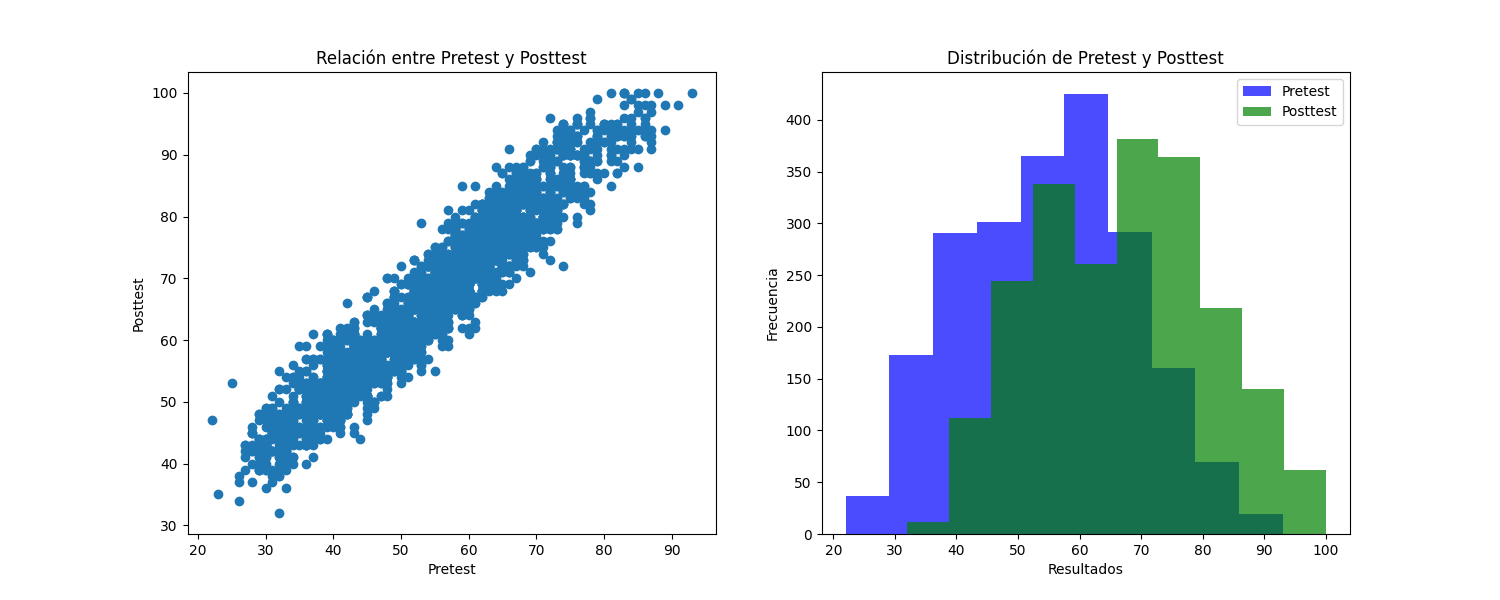
\includegraphics[width=1\textwidth]{images/relacion_pre_post.png}
    \caption{Relación lineal positiva entre Pretest y Posttest y sus distribuciones.}
    \label{fig:scatter}
\end{figure}

También se analizaron los diagramas de caja (boxplots) para detectar posibles valores atípicos y comparar las medianas y dispersión de ambas pruebas.

\begin{figure}[H]
    \centering
    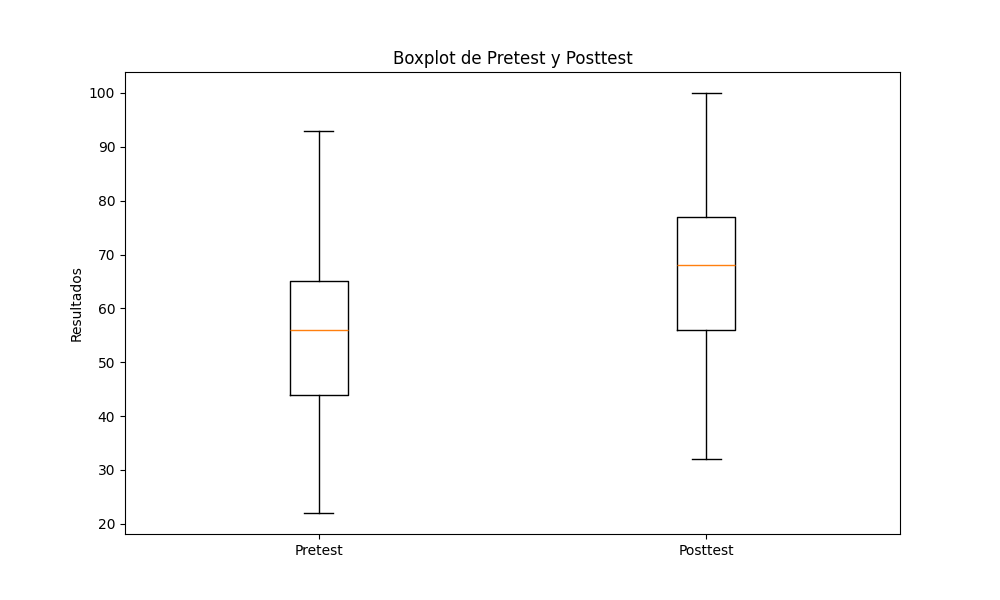
\includegraphics[width=0.7\textwidth]{images/boxplot_pre_post.png}
    \caption{Boxplot comparativo de puntajes Pretest y Posttest.}
    \label{fig:boxplot}
\end{figure}

Finalmente, se revisó la distribución de las variables categóricas demográficas para entender la composición de la muestra estudiantil.

\begin{figure}[H]
    \centering
    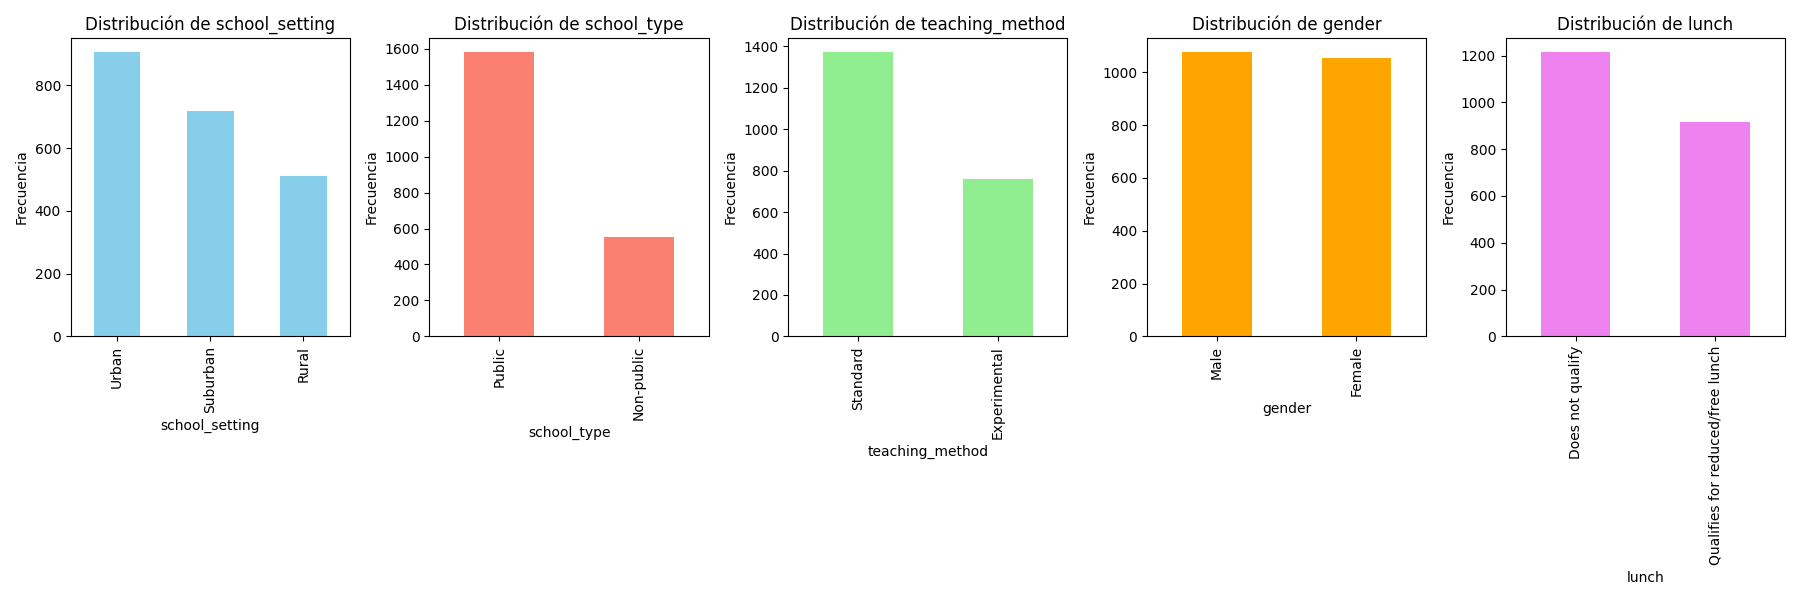
\includegraphics[width=1\textwidth]{images/distribucion_demografica.png}
    \caption{Distribución de variables demográficas en el dataset.}
    \label{fig:demographics}
\end{figure}

\subsection{Preprocesamiento}
Para preparar los datos para el modelo, se seleccionaron las variables más relevantes, descartando identificadores únicos como \texttt{student\_id} o \texttt{classroom} que no aportan valor predictivo generalizable.

Las variables categóricas fueron transformadas utilizando \texttt{pd.get\_dummies}, convirtiéndolas en variables numéricas binarias.

\begin{lstlisting}[language=Python]
# Selección de características
X = df[['school', 'school_setting', 'school_type', 
        'teaching_method', 'gender', 'lunch', 'pretest']]
y = df['posttest']

# Codificación One-Hot
X_encoded = pd.get_dummies(X, columns=['school', 'school_setting', 
                           'school_type', 'teaching_method', 
                           'gender', 'lunch'])
\end{lstlisting}

Posteriormente, se dividieron los datos en conjuntos de entrenamiento (70\%) y prueba (30\%) para garantizar una evaluación honesta del modelo.

\begin{lstlisting}[language=Python]
X_train, X_test, y_train, y_test = train_test_split(X_encoded, y, test_size=0.3)
\end{lstlisting}

\subsection{Entrenamiento del Modelo}
Se instanció y entrenó un modelo de Regresión Lineal utilizando los datos de entrenamiento procesados.

\begin{lstlisting}[language=Python]
model = LinearRegression()
model.fit(X_train, y_train)
\end{lstlisting}

% RESULTADOS
\section{Resultados}

\subsection{Métricas de Desempeño del Modelo Principal}
El modelo principal, que incluye todas las variables demográficas y el puntaje del pretest, mostró un desempeño excelente. Al evaluar el modelo con el conjunto de prueba, se obtuvieron los siguientes resultados:

\begin{itemize}
    \item \textbf{Coeficiente de Determinación ($R^2$):} 0.95. Esto indica que el modelo es capaz de explicar el 95\% de la variabilidad en los puntajes del examen final.
    \item \textbf{RMSE:} 3.12. En promedio, las predicciones del modelo se desvían aproximadamente 3 puntos del puntaje real.
\end{itemize}

\subsection{Análisis de Predicciones}
Al graficar los valores reales contra los valores predichos, se observa una alineación muy cercana a la diagonal ideal, lo que confirma la alta precisión del modelo. Los residuos (diferencias entre valor real y predicho) son bajos y no muestran patrones evidentes que sugieran sesgos sistemáticos.

\begin{figure}[h]
    \centering
    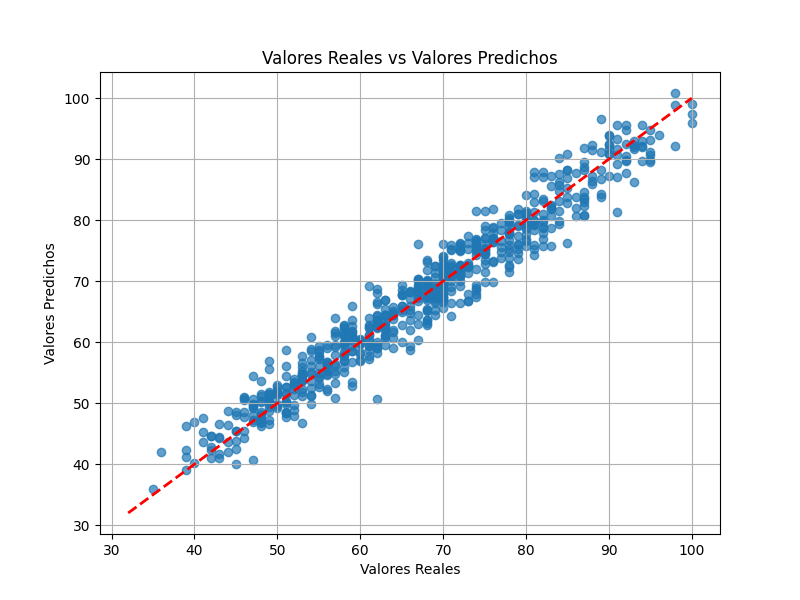
\includegraphics[width=0.7\textwidth]{images/reales_vs_predichos.png}
    \caption{Comparación entre valores reales y valores predichos por el modelo.}
    \label{fig:reales_vs_predichos}
\end{figure}

\subsection{Comparación de Modelos}
Para determinar la importancia de las diferentes variables, se realizaron experimentos con distintas configuraciones de variables. La siguiente tabla resume los resultados obtenidos:

\begin{table}[h]
\centering
\begin{tabular}{|l|c|c|c|}
\hline
\textbf{Modelo} & \textbf{Variables} & \textbf{$R^2$} & \textbf{RMSE} \\ \hline
Principal (Todas las variables) & 35 & 0.95 & 3.12 \\ \hline
Solo Pretest & 1 & 0.91 & 4.29 \\ \hline
Solo Demográfico (Sin Pretest) & 34 & 0.82 & 5.86 \\ \hline
Sin Escuela (Reducido) & 12 & 0.95 & 3.21 \\ \hline
\end{tabular}
\caption{Comparación de métricas entre diferentes modelos experimentales.}
\label{tab:comparacion}
\end{table}

Se puede observar que el modelo "Solo Pretest" por sí solo ya ofrece un $R^2$ muy alto (0.91), lo que confirma que el desempeño previo es el mejor predictor del desempeño futuro. Sin embargo, agregar información demográfica mejora el modelo hasta 0.95.

Es notable que el modelo "Sin Escuela", que elimina la variable específica del nombre de la escuela (reduciendo significativamente la dimensionalidad del modelo de 35 a 12 variables), mantiene un desempeño casi idéntico al modelo principal ($R^2$ de 0.95). Esto sugiere que las características generales de la escuela (\texttt{school\_setting}, \texttt{school\_type}) son suficientes para capturar el efecto del entorno escolar, sin necesidad de conocer el nombre específico de la institución.


% CONCLUSIONES
\section{Conclusiones}
En este proyecto se logró desarrollar con éxito un modelo de regresión lineal múltiple capaz de predecir los puntajes de exámenes escolares con una alta precisión ($R^2 = 0.95$). A través del análisis exploratorio y la experimentación con diferentes conjuntos de variables, se llegaron a las siguientes conclusiones clave:

\begin{enumerate}
    \item \textbf{El desempeño previo es el factor más determinante:} La variable \texttt{pretest} es, por mucho, el predictor más fuerte. Un modelo basado únicamente en esta variable ya alcanza un $R^2$ de 0.91.
    \item \textbf{El contexto demográfico importa:} Aunque el pretest es dominante, la inclusión de variables demográficas y del entorno escolar (como el tipo de escuela, método de enseñanza y subsidio de almuerzo) permite refinar las predicciones, reduciendo el error cuadrático medio de 4.29 a 3.12 puntos.
    \item \textbf{Generalización y Simplicidad:} Se demostró que no es necesario incluir el nombre específico de la escuela para obtener buenas predicciones. El modelo reducido, que utiliza solo las características generales de la escuela y el alumno, es igual de efectivo que el modelo completo pero mucho más simple y generalizable a nuevas instituciones.
\end{enumerate}

El modelo final representa una herramienta robusta para estimar el rendimiento académico, permitiendo identificar potencialmente a estudiantes que podrían necesitar apoyo adicional basándose en su perfil y resultados previos.

% REFERENCIAS BIBLIOGRÁFICAS
\begin{thebibliography}{99}

\bibitem{sklearn_lr}
Scikit-learn developers, ``sklearn.linear\_model.LinearRegression,'' \textit{Scikit-learn documentation}. [Online]. Available: \url{https://scikit-learn.org/stable/modules/generated/sklearn.linear_model.LinearRegression.html}. [Accessed: Nov. 22, 2025].

\bibitem{pandas_dummies}
The pandas development team, ``pandas.get\_dummies,'' \textit{pandas documentation}. [Online]. Available: \url{https://pandas.pydata.org/docs/reference/api/pandas.get_dummies.html}. [Accessed: Nov. 25, 2025].

\bibitem{sklearn_r2}
Scikit-learn developers, ``sklearn.metrics.r2\_score,'' \textit{Scikit-learn documentation}. [Online]. Available: \url{https://scikit-learn.org/stable/modules/generated/sklearn.metrics.r2_score.html}. [Accessed: Nov. 22, 2025].

\bibitem{sklearn_mse}
Scikit-learn developers, ``sklearn.metrics.mean\_squared\_error,'' \textit{Scikit-learn documentation}. [Online]. Available: \url{https://scikit-learn.org/stable/modules/generated/sklearn.metrics.mean_squared_error.html}. [Accessed: Nov. 22, 2025].

\end{thebibliography}

\end{document}
